\externaldocument{impl}

\chapter{Results and Discussion}
\label{chap:evaluation}

As a result of the ETL-Application a database with structured information about the national council is now available and can be used for further purposes. This database has been used for analysis and the results got visualized via a web application which is accessible for everybody. Figure \ref{fig:start_page_prototype} shows the start page of this application. Furthermore, the relation graphs of several periods get discussed in the sections \ref{sec:relations_clubs} and \ref{sec:relations_pol}. 

\begin{figure}
	\center
	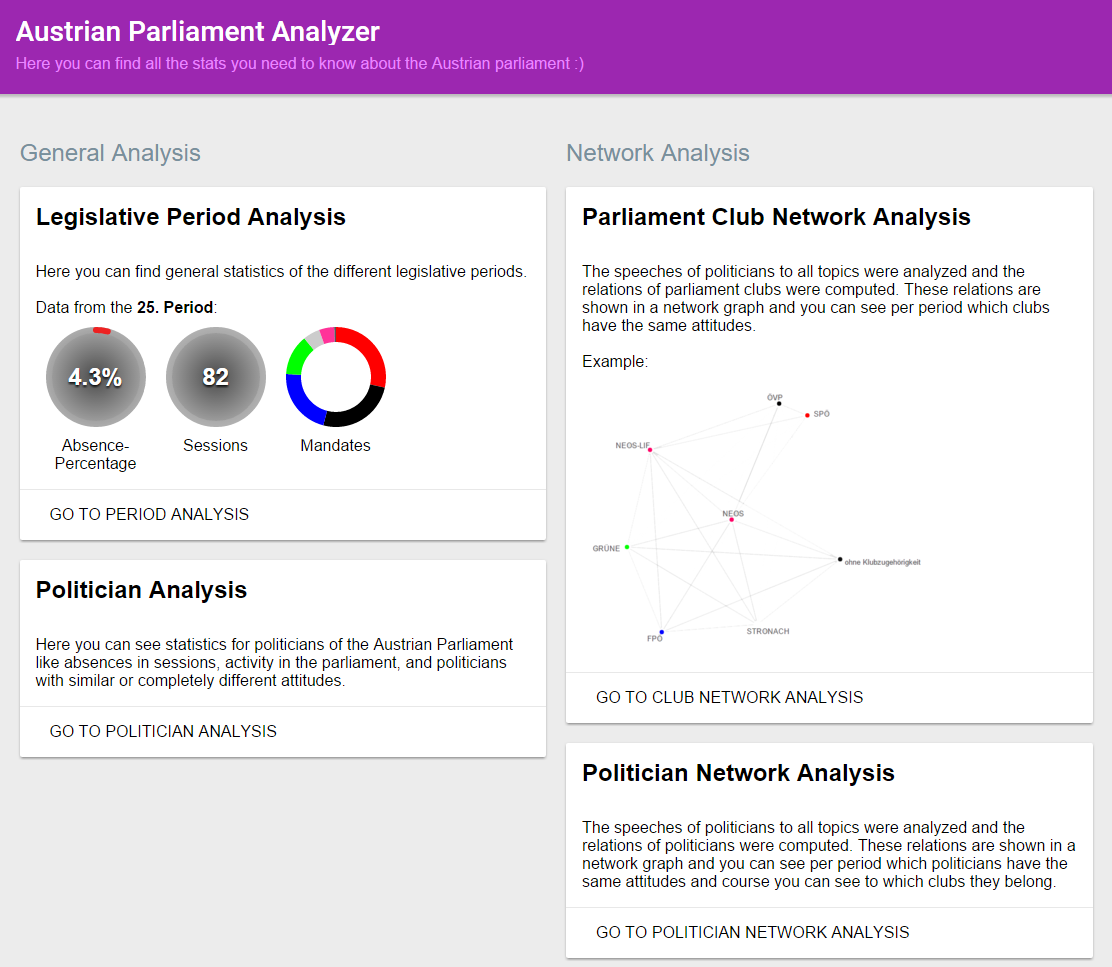
\includegraphics[width=0.75\textwidth]{imgs/result_start_page}
	\caption{Start Page of the Prototype Web Application}
	\label{fig:start_page_prototype}
\end{figure}

\section{Simple Analysis Results}
Table \ref{tab:simple_analysis_results} shows the results of some of the simple analysis measures, described in section \ref{sec:analysis}. The overall absence shows how often politician were absent during a certain period. Furthermore the table shows the most absent club and the most active politician for each discussed period (political activity is defined as how often a politician spoke in a discussion during a certain legislative period).

\begin{table}

\centering
\bgroup
\def\arraystretch{1.2}
\begin{tabular}{| p{2cm} | p{2cm} | p{3.5cm} | p{4cm} |}
\hline
  Legislative Period & Overall Absence & Most Absent Club & Most active Politician  \\
\hline
\hline
  20. Period & 2.8\% & Linke - 6.1\% & Volker Kier - 311 speeches \\
\hline
  21. Period & 2.7\% & Grüne - 4.6\% & Karl Öllinger - 216 speeches \\
\hline
  22. Period & 2.2\% & BZÖ - 5.6\% & Karl Öllinger - 227 speeches \\
\hline
  23. Period & 2.7\% & FPÖ - 6.0\% & Sigisbert Dolinschek - 108 speeches \\
\hline
  24. Period & 3.6\% & STRONACH - 7.0\% & Werner Kogler - 231 speeches \\
\hline
  25. Period & 4.2\% & STRONACH - 5.9\% & Gerald Loacker - 94 speeches \\
\hline

\end{tabular}
\egroup

\caption{Simple Analysis Measure Results}
\label{tab:simple_analysis_results}
\end{table}

\section{Relations of Parliament Clubs}
\label{sec:relations_clubs}
Figure \ref{fig:club_graphs1} shows the created relation graphs of the parliamentary clubs of the legislative periods 22 to 25. The graphs visualize the relations among the clubs through the distance between the nodes. The more positive the relation between two clubs is, the closer they appear together in the graph and the thicker is the edge between them. Only positive edges are shown in the graph, as the graph would look too confusing and messy if the negative edges were also shown. 

In all graphs shown, one can easily see that there are always two main groups of parliamentary clubs visible in the parliament: Those which are in government and those which are in opposition. In table \ref{table:gov_opp_parties} the parties are listed per period weather they were in government or in opposition. 
In the current period (25.) you can see that the governing parties (ÖVP and SPÖ) have a strong positive relationship and that there are only minor positive relationships between the governing parties and the NEOS party. All other parties in the opposition have negative relationships to the government. The graphs of the 24. and 24. period have a similar structure. In period 22, the government consists of ÖVP, FPÖ and BZÖ and there are again two groups of clubs in the graph, which are closely related. This shows that the distinctness of government and opposition does not depend on the composition of the parties which are in government or opposition.  

\begin{figure}
%\begin{tabular}{ c  c }
%	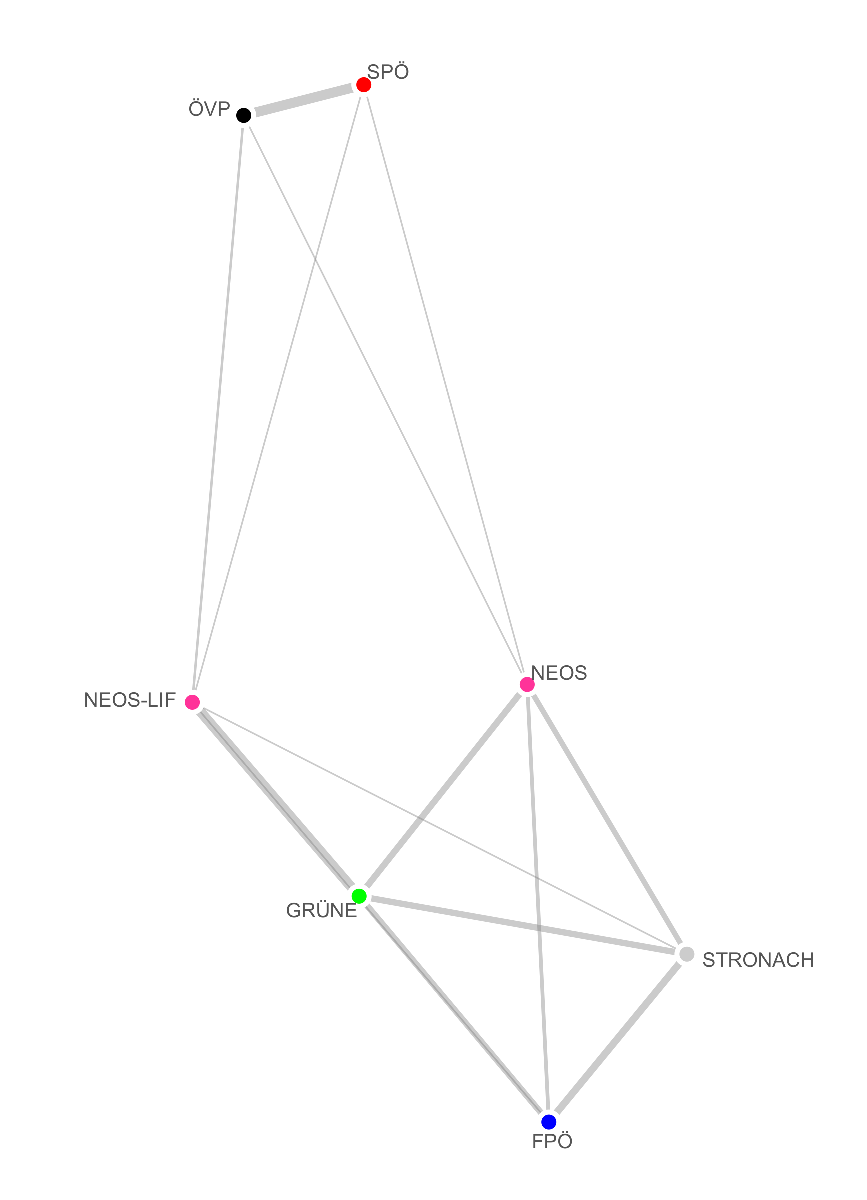
\includegraphics[width=0.47\textwidth]{imgs/graphs/club-graphs/graph_25.eps} 
	%& 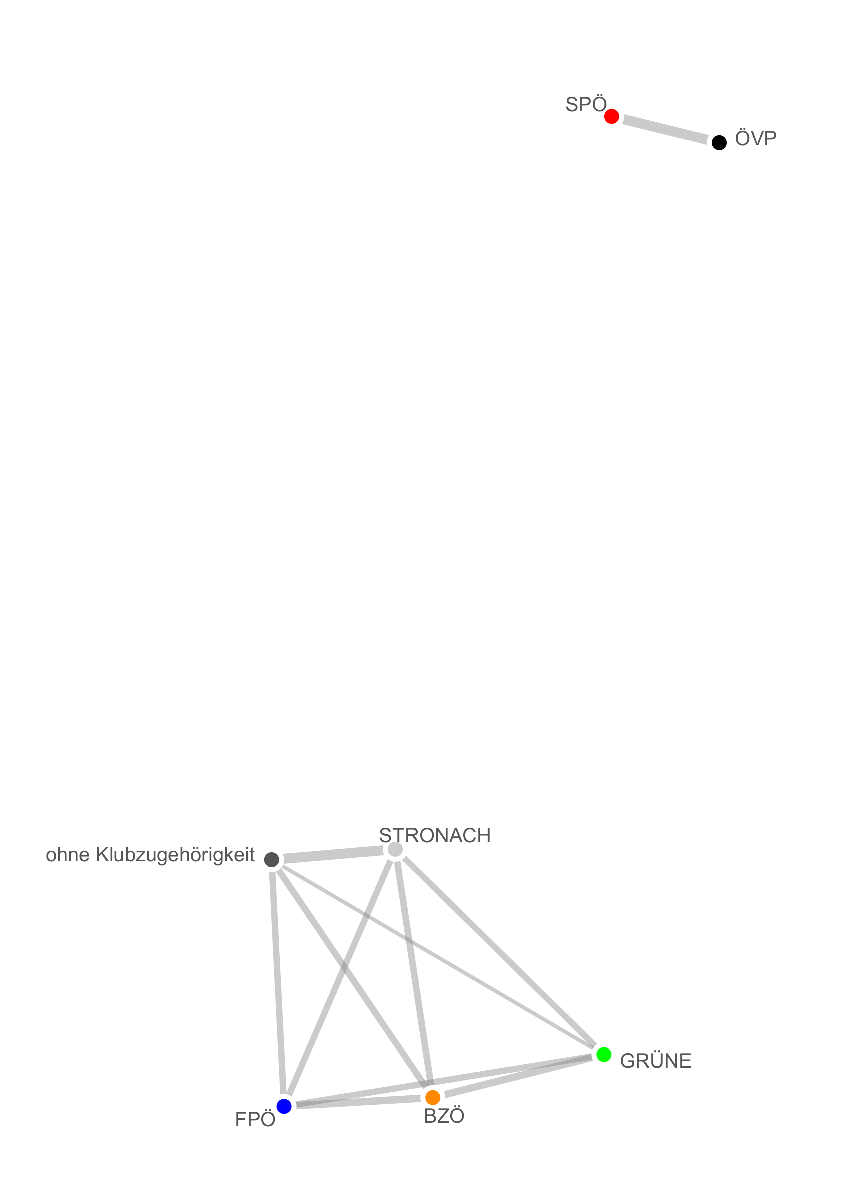
\includegraphics[width=0.3\textwidth]{imgs/graphs/club-graphs/graph_24.eps} 
%	& 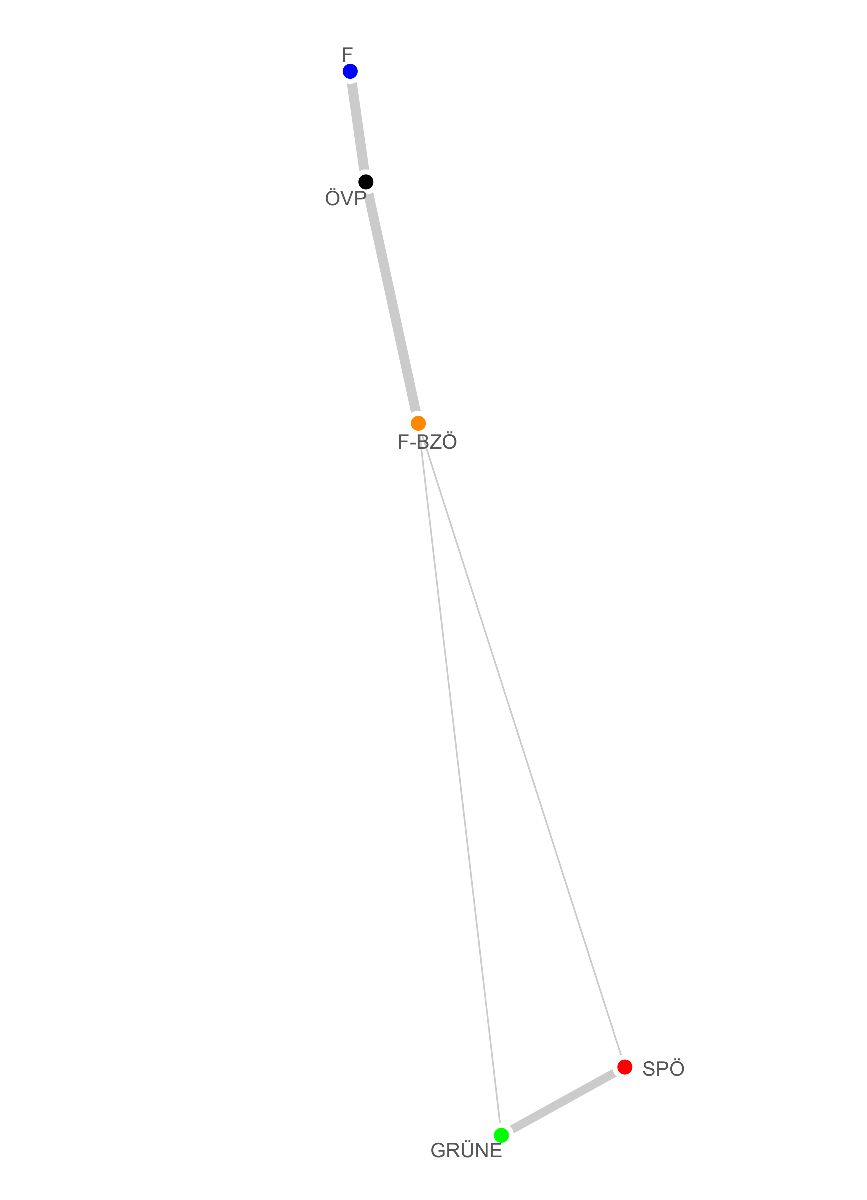
\includegraphics[width=0.47\textwidth]{imgs/graphs/club-graphs/graph_22.eps}
%	\\
%	(a) 25. Period 
	%& (b) 24. Period 
%	& (c) 22.Period
%\end{tabular}
	\center
	\setlength{\tabcolsep}{.26667em}
	\begin{tabular}{ c | c }
		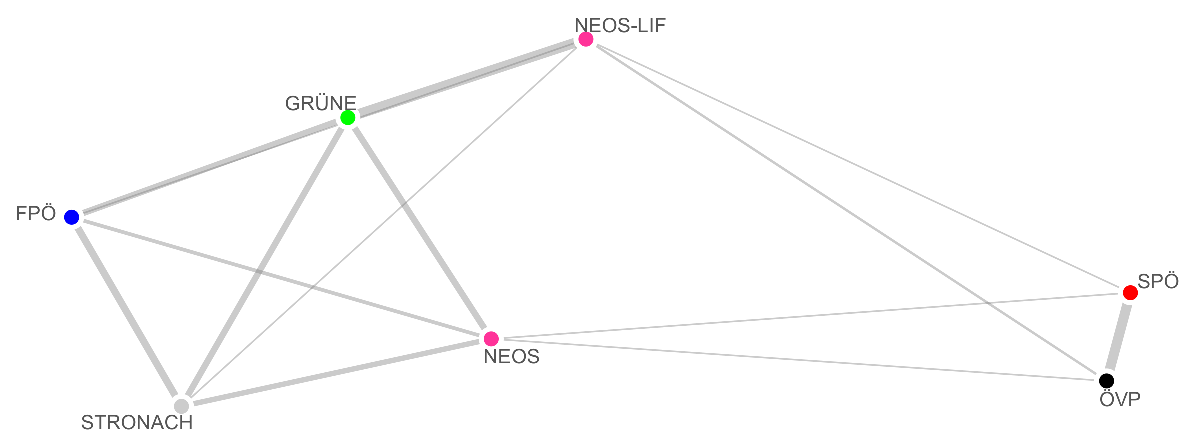
\includegraphics[width=0.48\textwidth]{imgs/graphs/club-graphs/horizontal/graph_25.eps}
		&
		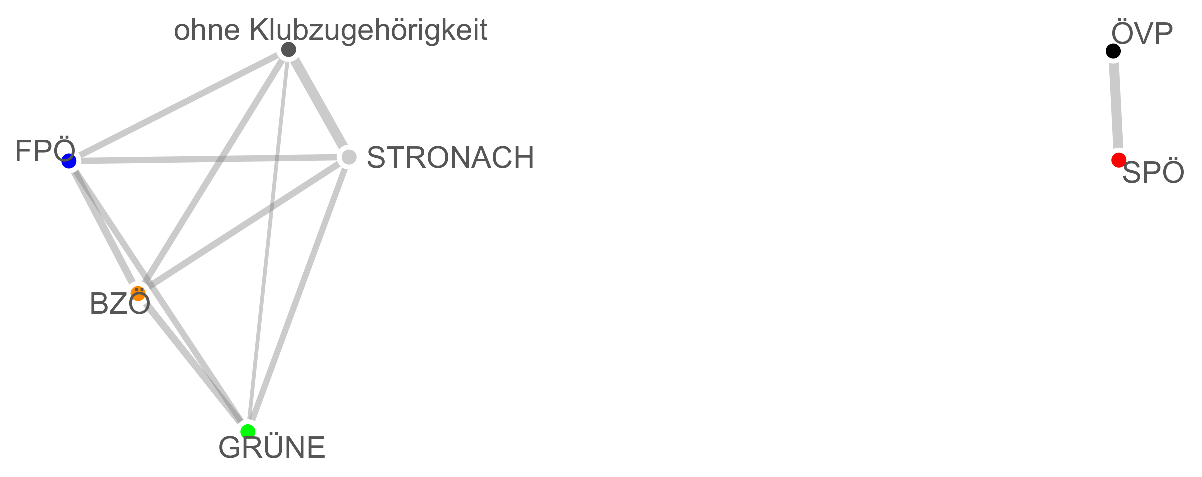
\includegraphics[width=0.48\textwidth]{imgs/graphs/club-graphs/horizontal/graph_24.eps}
		\\
		(a) 25. period
		&
		(b) 24. period
		
		\\
		\\
		\hline
		\\
		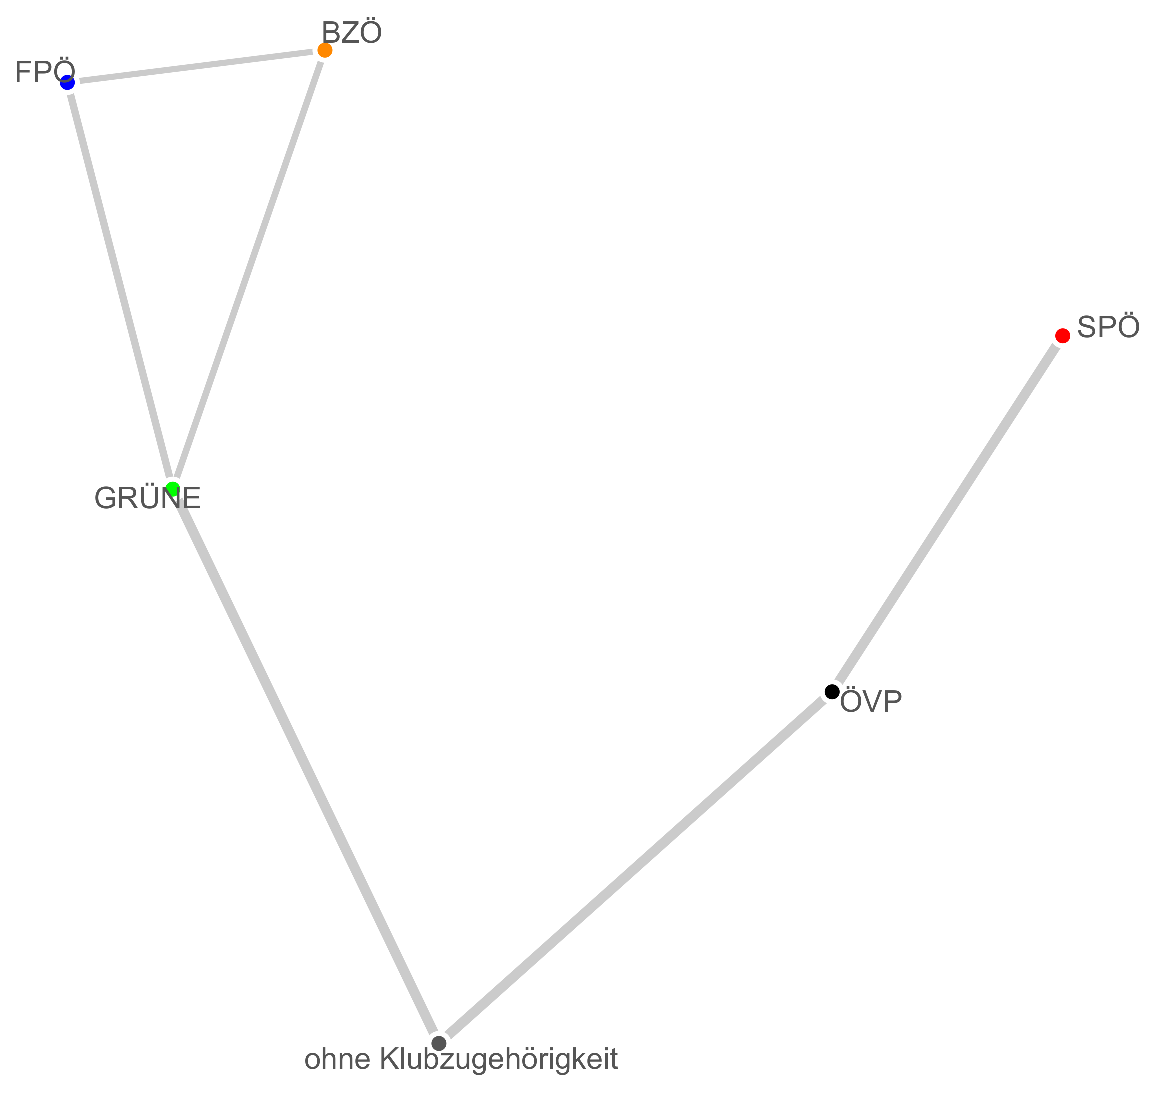
\includegraphics[width=0.48\textwidth]{imgs/graphs/club-graphs/horizontal/graph_23.eps}
		&
		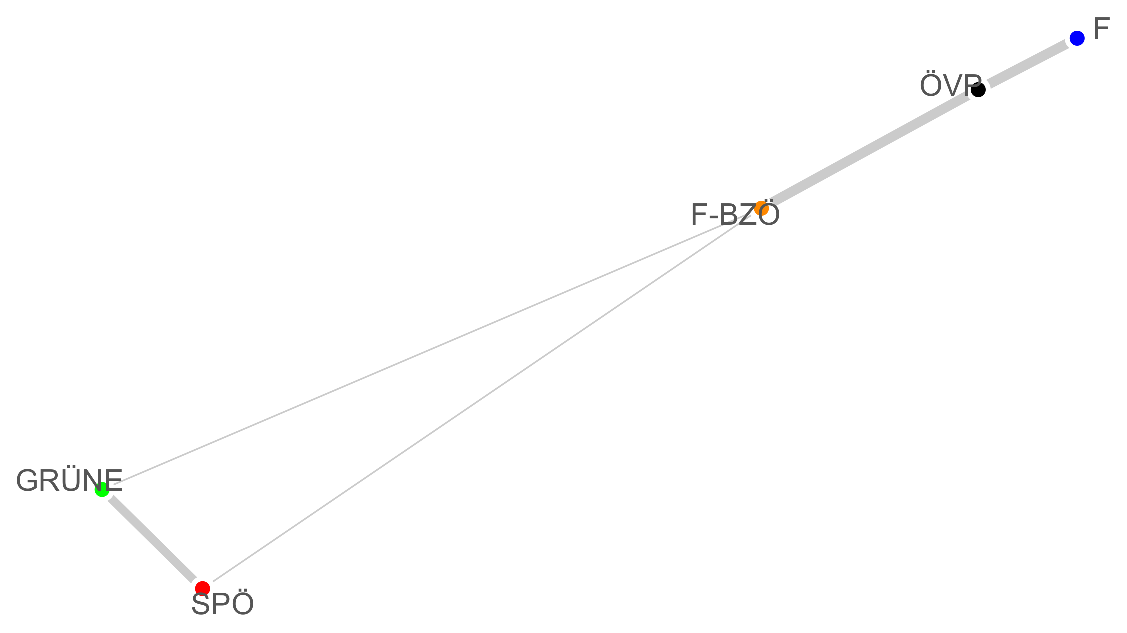
\includegraphics[width=0.48\textwidth]{imgs/graphs/club-graphs/horizontal/graph_22.eps}
		\\
		(c) 23. period
		&
		(d) 22. period
		\\
		\\
				
		
	\end{tabular}
	\todo{soll ich da auch noch 21. und 20. periode reingeben?}

	\caption{Club Relation Graphs}
	\label{fig:club_graphs1}
\end{figure}

\begin{table}

\centering
\bgroup
\def\arraystretch{1.2}
\begin{tabular}{| p{4cm} | p{3cm} | l |}
\hline
  Legislative Period & Governing Parties & Opposition  \\
\hline
\hline
  20. Period: 1995 - 1999 & SPÖ, ÖVP & FPÖ, Grüne, Liberale \\
\hline
  21. Period: 1999 - 2002 & ÖVP, FPÖ & SPÖ, Grüne \\
\hline
  22. Period: 2002 - 2006 & ÖVP, FPÖ, BZÖ\footnote{The BZÖ was in government from $17^{th}$ of April, 2005} & SPÖ, Grüne \\
\hline
  23. Period: 2006 - 2008 & SPÖ, ÖVP & FPÖ, Grüne, BZÖ \\
\hline
  24. Period: 2008 - 2013 & SPÖ, ÖVP & FPÖ, Grüne, Stronach, BZÖ \\
\hline
  25. Period: since 2013 & SPÖ, ÖVP & FPÖ, Grüne, NEOS, Stronach \\
\hline

\end{tabular}
\egroup
\caption{Government and Opposition in the Legislative Periods 20 to 25}
\label{table:gov_opp_parties}
\end{table}


\section{Relations of Politicians}
\label{sec:relations_pol}
Similar graphs to the ones in section \ref{sec:relations_clubs} were created for politicians. Figure \ref{fig:pol_graphs1} shows these graphs which have nodes for each active politician in the legislative periods 22 and 25. The closer two politicians appear together in a graph, the more positive is their relation. The politician nodes are in the color of the parliamentary club, the politician belongs to in the corresponding legislative period. The edges are colored in the color of the parliamentary club, if both politicians belong to the same club.

In the resulting graphs is again visible that the government and the opposition are two distinct groups. In the 25. period ÖVP (black) and SPÖ (red) are in government whereas in the 22. period ÖVP (black), FPÖ (blue) and BZÖ (orange) are in government. In both periods goverment and opposition can be visually separated. Also within government and opposition the politicians of the same club are displayed closely together. This effect is bigger in the opposition as the inner cohesion in the government is higher\footnote{see section \ref{fig:gov_opp_relation}}.

\begin{figure}
\center
\begin{tabular}{ c }
	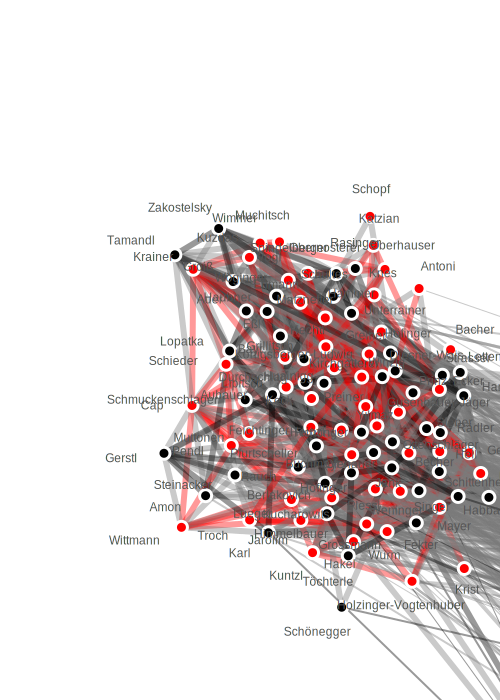
\includegraphics[width=0.85\textwidth]{imgs/graphs/politician-graphs/horizontal/graph_25.eps}
	\\
	(a) 25. Period
	\\
	\\
	\hline
	\\
	%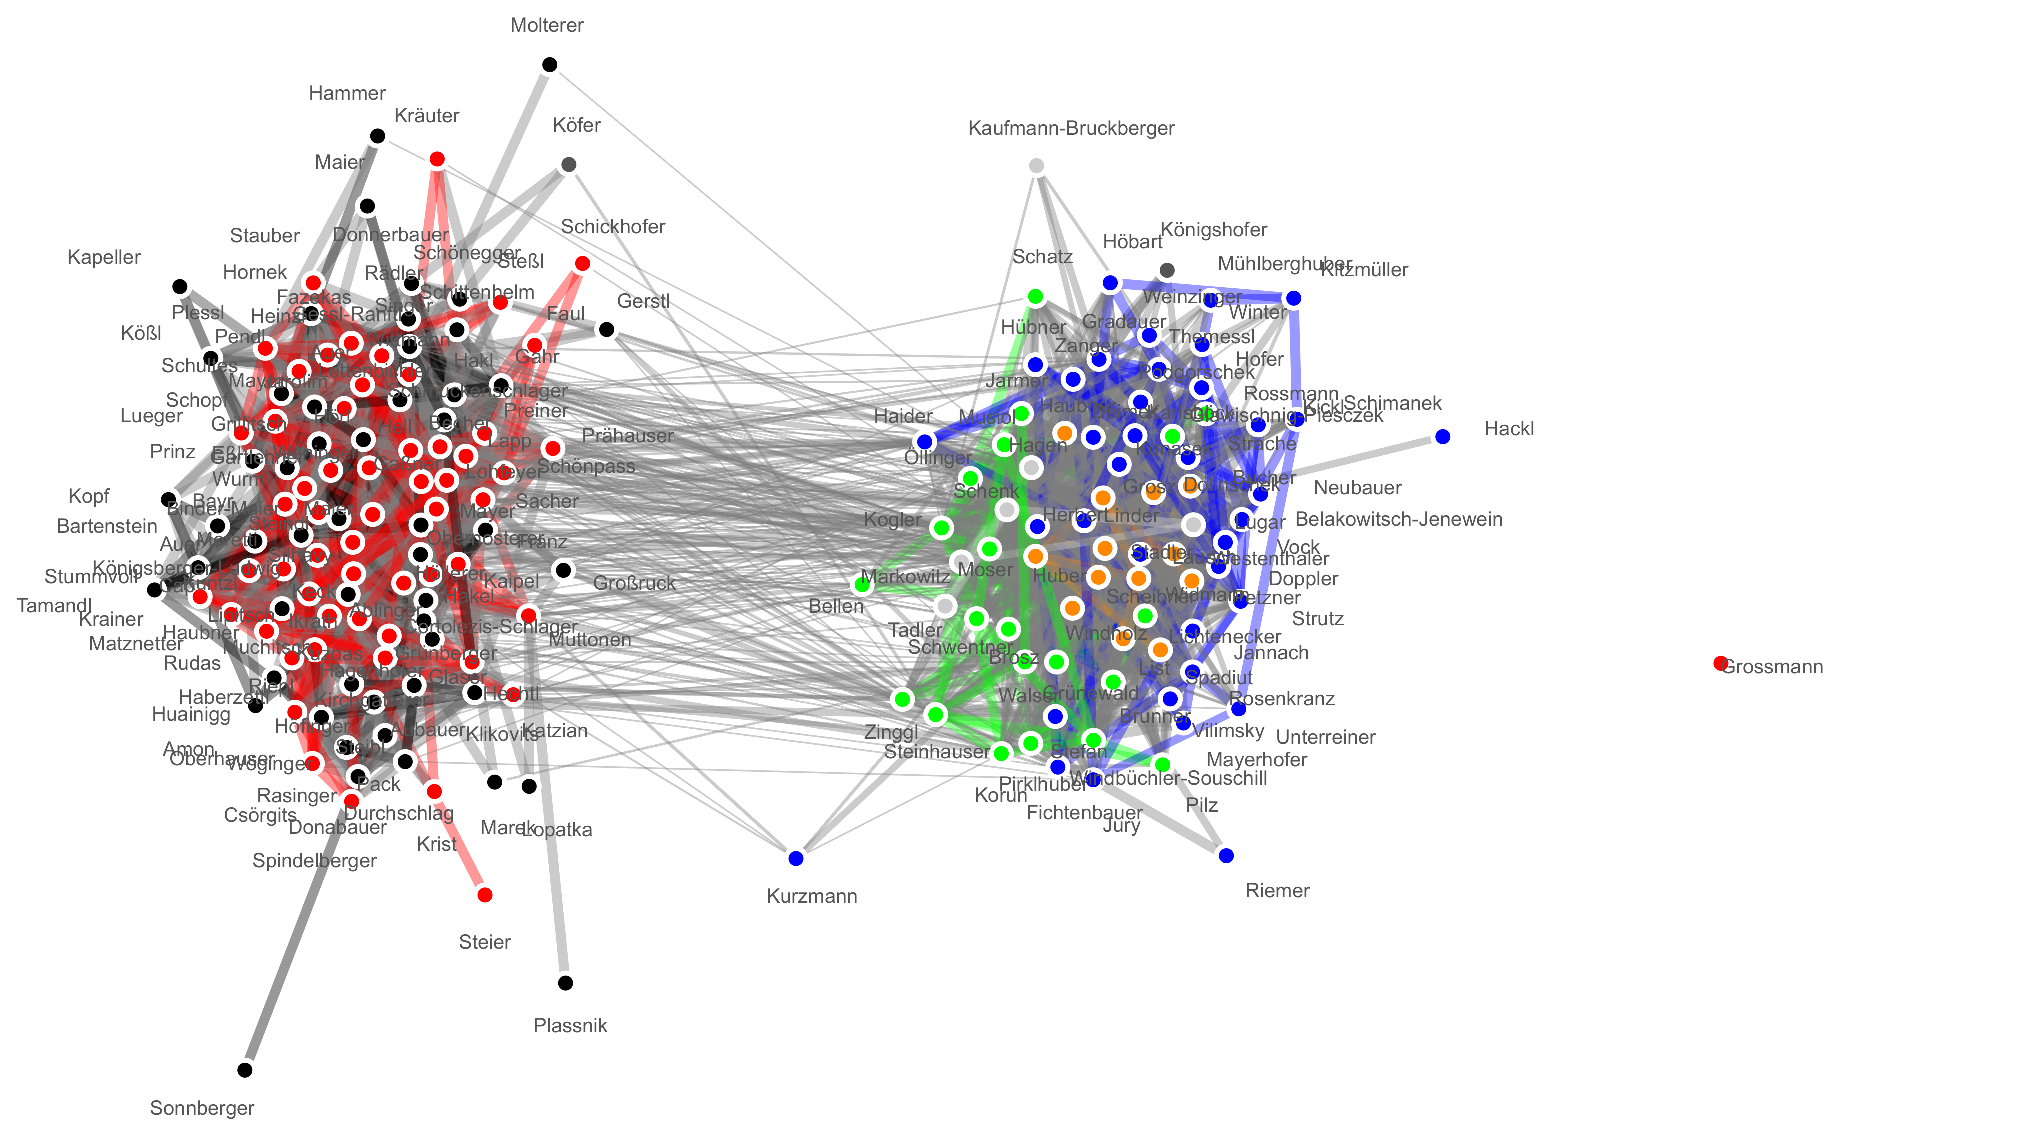
\includegraphics[width=0.7\textwidth]{imgs/graphs/politician-graphs/horizontal/graph_24.eps}
	%\\
	%(b) 24. Period
	
	%\\
	%\hline
	%\\
	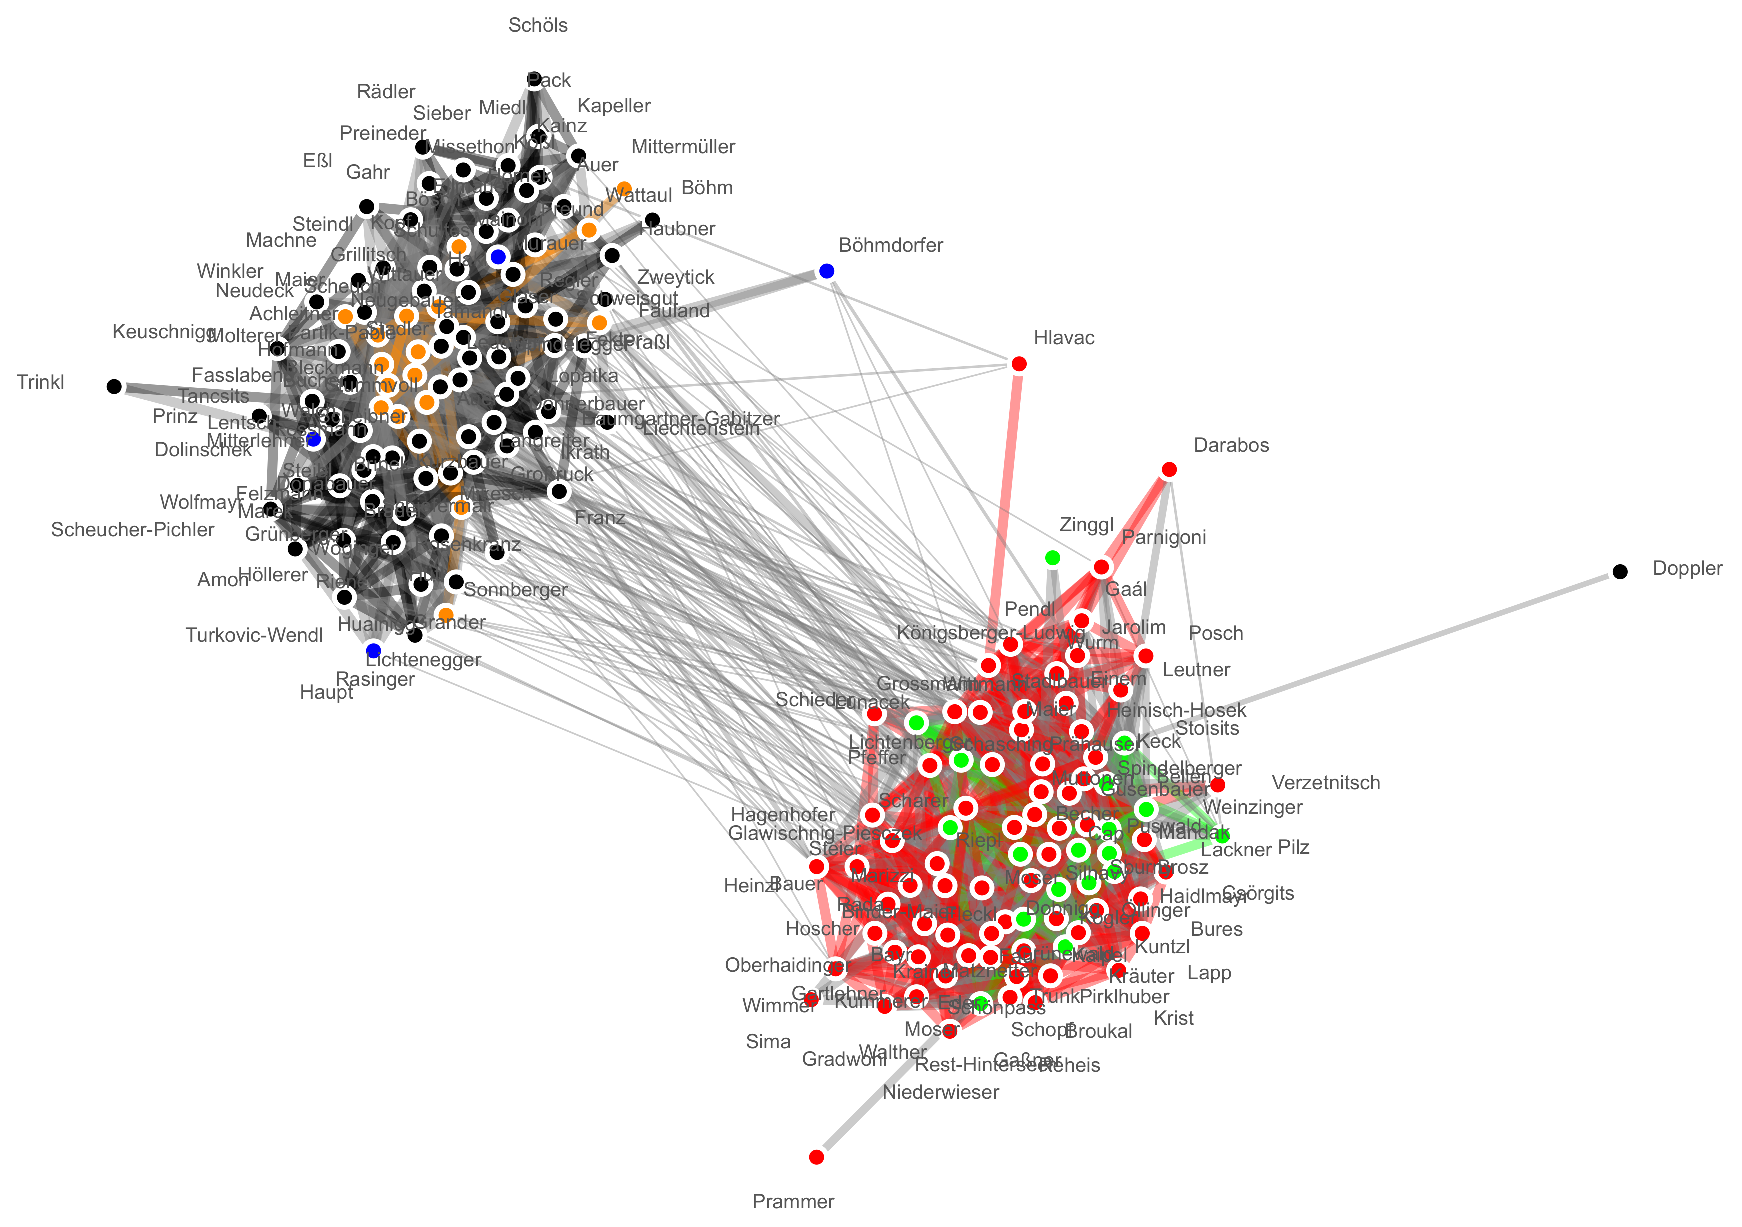
\includegraphics[width=0.85\textwidth]{imgs/graphs/politician-graphs/horizontal/graph_22.eps}
	\\
	(b) 22. Period
\end{tabular}
	
	
	\caption{Politician Relation Graphs}
	\label{fig:pol_graphs1}
\end{figure}

\section{Government - Opposition Relation}
\label{sec:gov_opp_relation}
Table \ref{table:gov_opp_relation} shows the results of the measures taken for the government-opposition relation, inner government cohesion and inner opposition cohesion. Figure \ref{fig:gov_opp_relation} shows the changes over time of these values. The values show that the two main groups in the parliament - the government and opposition - are highly distinct. The government-opposition relation is negative in every discussed period. This means that there is an overall tendency of politicians in government and opposition to have different opinions. The values differ in the periods, the 20. period shows a the most negative value with $-0.85$. This means that only in $7.5$\% of the speeches a politician in government and one in opposition had the same opinion on a certain topic, in all other speeches they had contrary ones. In the current period, this inter relationship value is still negative, but the negative relationship is a lot less significant. The relation coefficient is $-0.374$ which means that in $31.3$\% of the speeches government and opposition have the same opinion.

The inner-government cohesion shows how homogeneous the attitudes of all politicians in government is. In all analyzed legislative periods, the cohesion is almost $+1.00$ which means that almost all politicians had the same opinions on all topics spoken in. Analogously to the inner-government cohesion the inner-opposition cohesion shows the cohesion within the opposition and how homogeneous their attitudes were. The resulting cohesion values were more interesting because they varied in the analyzed periods. The values were in the range of $+0.938$ to $+0.676$. In the period, with the highest inner opposition cohesion (period 22), in 96.6\% of the speeches the politicians in opposition had the same opinion. In the current period, the opposition cohesion coefficient is $+0.676$. This means that 83.8\% of the politicians in opposition had the same attitudes on the discussions they spoke in.

There is a general tendency visible that the inner-opposition cohesion decreased over the last legislative periods and the government-opposition relation became less and less negative. This could be caused by a more diverse parliament - in the recent periods there were more different clubs in opposition. Obviously, this leads to a lower inner-opposition cohesion. For example, if there would be only one party in opposition, the cohesion would be virtually 1.00, but if there would be a lot more, the cohesion would decrease dramatically.

\begin{table}

\centering
\bgroup
\def\arraystretch{1.2}
\begin{tabular}{| p{2cm} | p{3cm} | p{3cm} | p{3cm} |}
\hline
  Legislative Period & Government-Opposition Relation & Inner-Government Cohesion & Inner-Opposition Cohesion \\
\hline
\hline
  20. Period & $-0.85$ & +1.00 & +0.86 \\
\hline
  21. Period & $-0.695$ & +0.985 & +0.908 \\
\hline
  22. Period & $-0.567$ & +1.00 & +0.938 \\
\hline
  23. Period & $-0.382$ & +0.994 & +0.765\\
\hline
  24. Period & $-0.52$ & +1.00 & +0.768\\
\hline
  25. Period & $-0.374$ & +1.00 & +0.676\\
\hline

\end{tabular}
\egroup
\caption{Government-Opposition Relation, Inner Government- and Inner Opposition Relation for the Legislative Periods 20 to 25}
\label{table:gov_opp_relation}
\end{table}

\begin{figure}
\center
	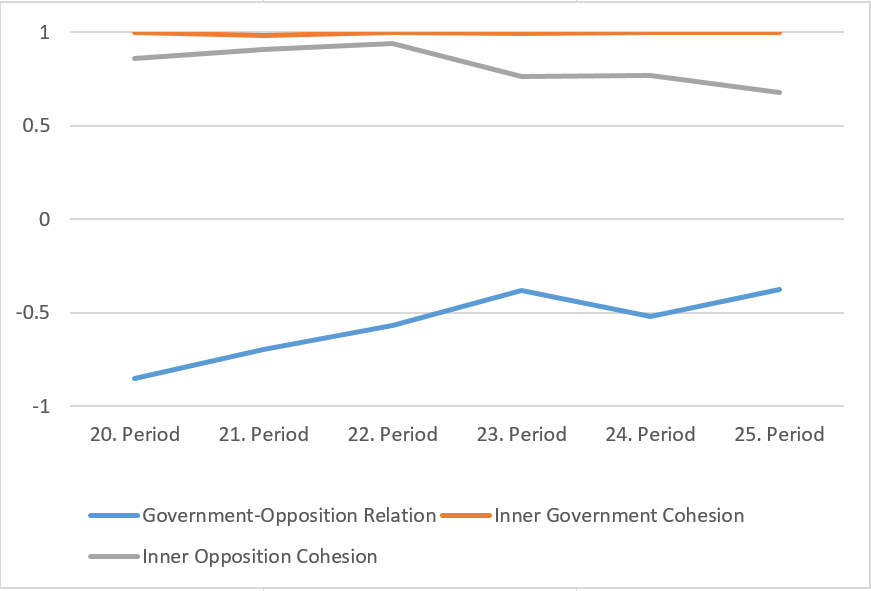
\includegraphics[width=0.75\textwidth]{imgs/gov_opp_rel_graph}
	\caption{Development of the Inter-Government-Opposition Relationship Coefficient and Inner Cohesion Values over Time}
	\label{fig:gov_opp_relation}
\end{figure}